% !TeX spellcheck = en_US
% !TeX encoding = UTF-8
% !TeX root = ../thesis.tex

\chapter{Swarm Reinforcement Learning with Graph Neural Networks}
\label{ch:Architecture}
% pages: 4.26-5.68
% ~966 words
First we will introduce the policy architecture used as the base. It is designed to work with PPO and uses the latent node features of the observation for the actor and critic. This base is then expanded with a Graph Neural Network structure that allows multiple hops through a stack of message passing blocks. To support heterogeneous graphs needed for tasks like pursuit the architecture is extended to work on multiple graphs as inputs, but it retains the overarching structure. This makes both GNNs interchangeable. Most of the changes needed for heterogeneous graphs is located in the edge-, node- and global-modules.



% ~322 words
\section{PPO - Policy Architecture}
\begin{figure}[htp]
    \centering
    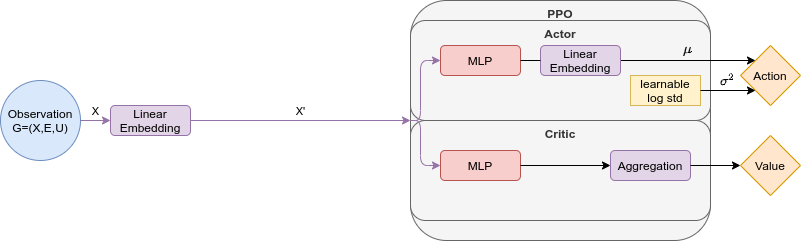
\includegraphics[width=1.0\textwidth]{figures/PPO_no_message_passing.png}
    \hspace{1cm}   
    \caption{Policy architecture used for Swarm Reinforcement Learning with Graph Neural Networks. The node features of the observation graph is the only data used. Here the actor and critic use the same embedding. It is put into a latent dimension and then used by the PPO Network to calculate the action as a distribution and the value.}
    \label{fig:PPO_no_message_passing}
\end{figure}

An overview of the policy architecture as desribed below can be seen in \Cref{fig:PPO_no_message_passing}.

Our environments can have different observations structured as a graph $G = (X,E,U)$. For now we will talk about homogeneous graphs. Each agent $a_k$ uses information it knows about itself and what it knows about it's neighboring agents $a_i \in \mathcal{N}_k$. The neighborhood is determined either by the culling method kNN or using the euclidean distance. The specific data for each environment is described in \Cref{ch:Experiments}. Information about $a_k$ is used as the node-features $x_k$ for the graph. The edges $E$ describe neighborhood relations for a given $\mathcal{N}_k$. For an edge $\{x_i,x_j\} = e \in E$ edge-features on the other hand describe the individual observations from $a_x$ about the state of the agent $a_y$. \Citet{RobinRuede2021} uses a similar observation structure implicitly. Edge-features are created using an $\textup{observe()}$ function. They explicitly calculate the neighborhood for each agent that uses the policy. \par

For testing and debugging purposes, the Graph Neural Network (GNN) can be disabled. When it is, only the node-features are used. Once the observation graph is constructed, the node-features are encoded into a latent-space representation. For this embedding we use a linear layer. We allow for independet embedding for the actor and critic. They can either share the same embedding or have different embeddings. The Multi-Layer Perceptron (MLP) used in \Citet{RobinRuede2021} is used as an encoding step and to process each element of an aggregation group. Processing is not needed for our embedding, as our GNN is responsible for that, so a simple linear transformation is enough.\par

The learning head for Proximal Policy Optimization (PPO) is composed of the actor describing the policy $\pi$, which gets us the joint action $\textup{act} = \langle \textup{act}_1,...,\textup{act}_n \rangle$ and the critic calculating the running advantage $A$. Our actor uses an MLP, followed by another linear transformation. It will reduce the dimension from the latent dimension back to the action dimension. This is then used as the mean $\mu$ for a diagonalized Gaussian distribution to support non deterministic policies. The variance $\sigma^2$ uses a learnable logarithmic standard deviation. The critic also uses an MLP with an output-dimension of 1. This defines a value per node in the graph. In \Citet{RobinRuede2021} the authors define a value for each agent. This helps to identify which agent was responsible for the reward. But this is not how the PPO Algorithm was originally designed to work for single-agent environments. Our architecture can use an aggregation to output a single value per graph. This can either be $\min(x)$, $\max(x)$, $\textup{mean}(x)$. Through exploration the agents are still able to identify over time how much an agent was responsible for a given reward. We parameterized node-wise values and graph-wise values for our approach. \par



% ~322 words
\section{Homogeneous Message-passing GNN Architecture}
\begin{figure}[htp]
    \centering
    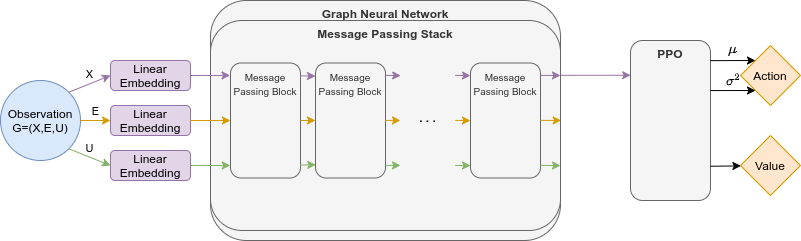
\includegraphics[width=1.0\textwidth]{figures/homogeneous_gnn.png}
    \hspace{1cm}   
    \caption{Here a GNN is added as a step before the policy architecture. The entire observation is put into a latent space and then passed through multiple message passing hops. The outputs of one hop is used as the input of the next hop. This is coordinated through the message passing stack.}
    \label{fig:homogeneous_gnn}
\end{figure}

An overview of the message passing architecture for homogeneous graphs as described below can be seen in \Cref{fig:homogeneous_gnn}.

When enabling the GNN, it is added as a step between the policy architecture and observation. node-features, edge-features and global-features are now embedded into a latent-space linearly similar to above. The weights between the encoders are not shared. Global-features can be used to explicitly give the swarm global information. In our experiments this was not needed. \par

We choose to use a GNN structure that uses stacks of GNN blocks. Each block defines a single message-passing hop. The stack is an array of blocks that are used sequentially. This way we are able to support multiple GNN hops. We do want to note, that \Citet{RobinRuede2021} model architecture for a single aggregation group can be described via the function:

\begin{equation}
    f(a_i) = \textup{decoder(selfObserve}(a_i), \underset{j \in \mathcal{N}_i}{\oplus}\ \textup{encoder}(\textup{observe}(a_i, a_j))) \nonumber
\end{equation}

As can be seen, this already implements a common message-passing GNN. In comparison our architecture adds the ability to process multiple GNN hops.
The GNN block is composed of an edge-, node-, and global-module, each responsible for the corresponding features. An diagram of the relationship between these blocks is outlined in \Cref{fig:message_passing_block}. The functions used by the modules are as following:

\begin{equation}
    \begin{aligned}
        \textup{Edge-Module:}\ & x_{e'} = f_e(x_v, x_u, x_e, x_g)\\
        \textup{Node-Module:}\ & x_{v'} = f_v(x_v, \oplus_{\{e'=(v,u)||_v\}} x_{e'}, x_g)\\
        \textup{Global-Module:}\ & x_{g'} = f_g(\oplus_V x_{v'}, \oplus_E x_{e'}, x_g)
    \end{aligned}
    \nonumber
\end{equation}

Similar to the embedding, our architecture allows for two GNN modules for the value and critc. Each of them have seperate embedding and a seperate GNN module. This allows both to process observations differently. Each of the aggregation functions used in the entire network are shared and can be set to $\min(x)$, $\max(x)$, or $\textup{mean}(x)$. Furthermore the input of a GNN block can be added to the output. These residual connections help with the vanishing/exploding gradients problems by breaking up the multiplications.

\begin{figure}[htp]
    \centering
    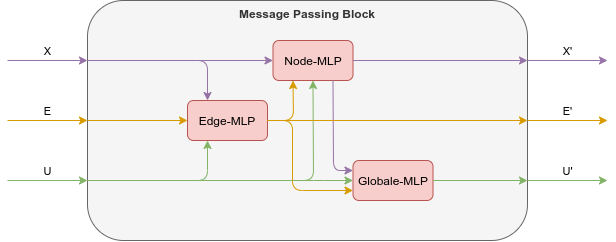
\includegraphics[width=0.75\textwidth]{figures/message_passing_block.png}
    \hspace{1cm}   
    \caption{This is a detailed view of one message passing block. It uses a edge-, node- and global-module to compute a single message passing hop.}
    \label{fig:message_passing_block}
\end{figure}



% ~322 words
\section{Heterogeneous Message-passing GNN Architecture}
\begin{figure}[htp]
    \centering
    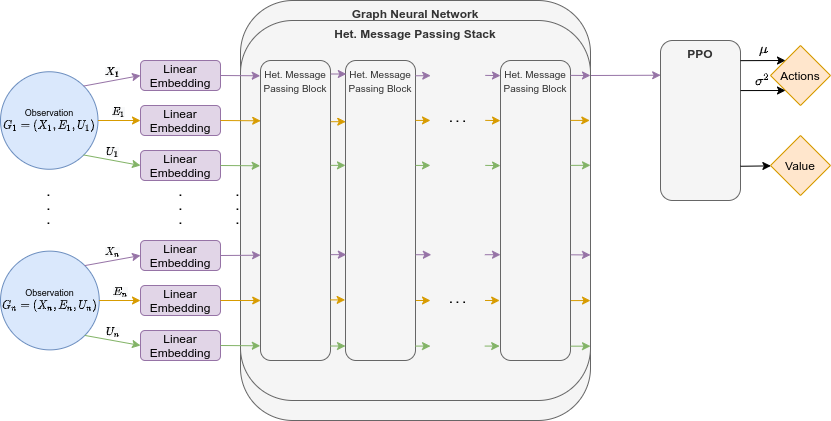
\includegraphics[width=1.0\textwidth]{figures/heterogeneous_gnn.png}
    \hspace{1cm}   
    \caption{An overview of the heterogeneous version of the architecture. The overall structure stays the same, but the input observation is now mulitple graphs. each of the input embeddings per graph is unique. The policy architecture only uses one of the note types as input.}
    \label{fig:heterogeneous_gnn}
\end{figure}

An overview of the message passing architecture for heterogeneous graphs as described below can be seen in \Cref{fig:heterogeneous_gnn}.

This extension is used when an environment needs multiple distinct information types. By using heterogeneous graphs we are able to support multiple aggregation Groups as in \Citet{RobinRuede2021}. An heterogeneous graph $G = (X, E, U)$ is composed of multiple node-types $X_i, i = 1,...,m$, where $X = \bigcup_{i=1}^m X_i$ and multiple edge-types $E_i, i = 1,...,m^2$, where $E = \bigcup_{i=1}^{m^2} E_i$. An edge-type is uniquely identified by its source node-type and destination node-type where $\forall E_i: \exists j,k \leq m: E_i = (V_j \times V_k)$. If the source- and destination-node-types are not the same i.e. $j \neq k$, we can either define the edge-types as directed, or make it undirected. In the undirected case not all node-type combinations are edge-types, because $(V_j \times V_k) = (V_k \times V_j)$. Here the edge-type of $(V_j \times V_k)$ is sufficient. in the directed case $(V_j \times V_k) \neq (V_k \times V_j)$ and both types are needed. For experiments, both variations are parameterized in our architecture. If $j = k$ the edge-type can be directed or undirected, which depends on the culling method used. \par

Each of the node-types and edge-types are linear embedded. Each type has it's own linear transformation. As different types define completely aggregation groups, weight sharing is not used. global features are also embedded independently. Structurely the heterogeneous GNN stacks and blocks are the same, they only have more inputs. The underlying heterogeneous edge-, node- and global-modules have the following functions:

\begin{equation}
    \begin{aligned}
        \textup{Edge-Module:}\ & x'_{e_i} = f_{e_i}(x_v, x_u, x_{e_i}, x_g), e_i = (u, v)\\
        \textup{Node-Module:}\ & x'_{v'_i} = f_{v_i}(x_{v_i}, [\otimes_j\ \oplus_{\{e_j=(v_i,u)\}} x'_{e_j}], x_g)\\
        \textup{Global-Module:}\ & x'_{g} = f_g([\otimes_j\ \oplus_{V_j} x'_{v\in V_j}], [\otimes_k\ \oplus_{E_k} x'_{e\in E_k}], x_g)
    \end{aligned}
    \nonumber
\end{equation}

In addition to the options outlined in the homogeneous GNN section, we are able to define different functions for $\otimes$ and $\oplus$. $\oplus$ follows the global aggregation function setting shared by the network. $\otimes$ on the other hand can be either defined as a concatenation or as the global aggregation function. \Citet{RobinRuede2021} only uses a concatenation. The concatenation is more expensive as the input dimension of the MLP of the node-, or global-module is larger. Though it is more expressive than the alternative of using aggregation. In tasks like multi evader pursuit, if the different node-types are aggregated, it is harder for agents to distinguish between the data that came from other agents or from the evaders.

\iffalse
An overview of the heterogeneous message passing block can be seen in \Cref{fig:heterogeneous_message_passing_block}.

\begin{figure}[htp]
    \centering
    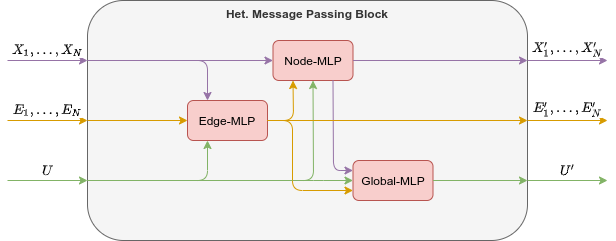
\includegraphics[width=0.85\textwidth]{figures/heterogeneous_message_passing_block.png}
    \hspace{1cm}   
    \caption{Also the structure of the message passing block stays similar. Now the three blocks take all the nodes, edges and global-features of all graphs as input and as output.}
    \label{fig:heterogeneous_message_passing_block}
\end{figure}
\fi
